
%===========================================================
% do not change this formatting please :-)
%===========================================================
\documentclass[letter,12pt]{article}
\usepackage[margin=1in]{geometry}
\usepackage{pdfpages}
\usepackage{amssymb,amsmath,amsthm,mathrsfs,colortbl,fancyhdr,tcolorbox,enumitem}
\fancyhead{}
\fancyhead[L]{Collin McDevitt} %Replace "NAME: " WITH YOUR NAME
\fancyhead[C]{MATH 5235 HOMEWORK 02}
\fancyhead[R]{PAGE \thepage}
\fancyfoot{}
\renewcommand{\footrulewidth}{0.4pt}

\date{\today}
%===========================================================
% convenient commands -- feel free to add more as you see fit
%===========================================================
\newcommand{\C}{\mathbb{C}}
\newcommand{\K}{\mathbb{K}}
\newcommand{\Poly}{\mathcal{P}}
\newcommand{\Q}{\mathbb{Q}}
\newcommand{\R}{\mathbb{R}}
\newcommand{\dotp}{\boldsymbol{\cdot}}
\begin{document}
\pagestyle{fancy}
%===========================================================
%===========================================================
%===========================================================
% PROBLEM 1
%===========================================================
\begin{tcolorbox}
   Define explicitly a continuous branch of $\log z$ in the complex plane slit along the negative imaginary axis, $\mathbb{C}\setminus[0,-i\infty).$
\end{tcolorbox}

This branch is given by $f(re^i\theta)=\log r+i\theta$ where $\theta \in (-\frac{\pi}{2},\frac{3\pi}{2})$.


\begin{tcolorbox}
    Sketch the image of the sector $\{0<\arg z<\frac{\pi}{6}\}$ under the map $w=z^a$. \begin{itemize}
        \item $a=\frac{3}{2}$
        \item $a=i$
    \end{itemize}
\end{tcolorbox}

$$w=z^\frac{3}{2}=e^{\frac{3}{2}(\log|z|+i\text{Arg}z)}=|z|^\frac{3}{2}e^{\frac{3}{2}i\text{Arg}z}$$





$$w=z^i=e^{i \log z}=e^{i(\log|z|+i\text{Arg}z)}=e^{-\text{Arg}z+i\log|z|}$$




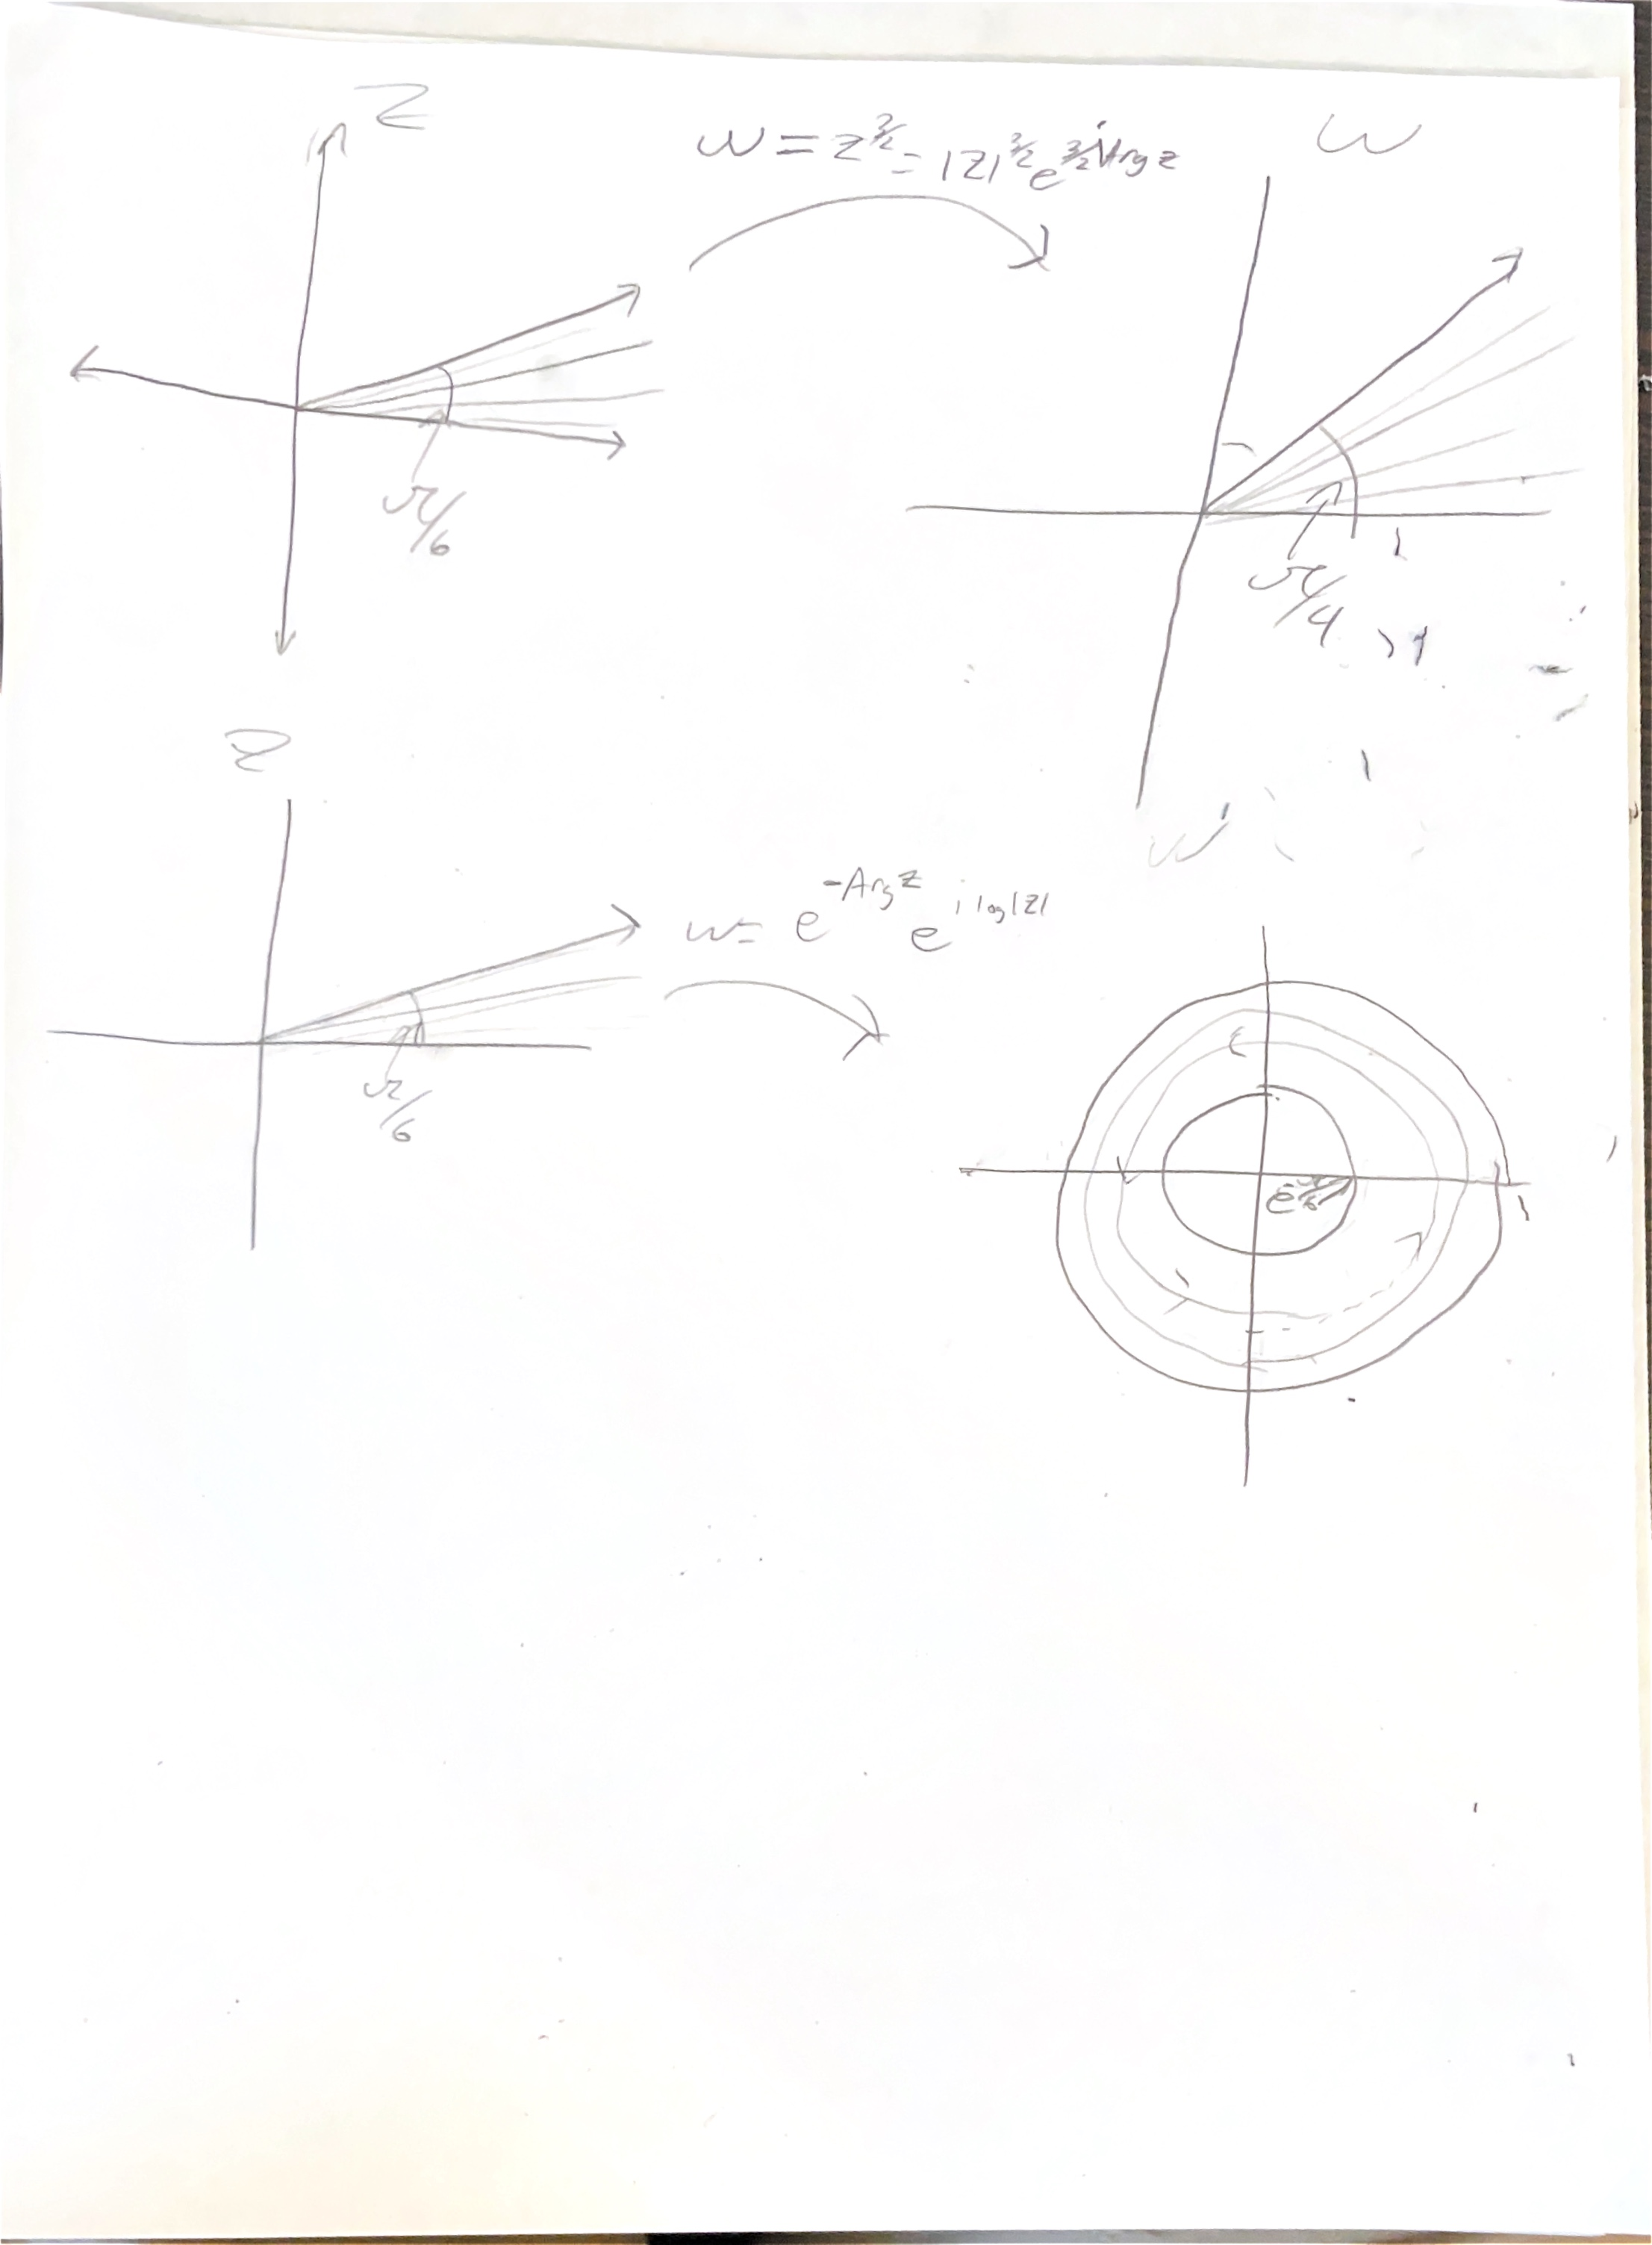
\includepdf[pages={1}]{Mappings.pdf}

\begin{tcolorbox}
    Determine the phase factors of the function $z^a(1-z)^b$ at the branch points $z=0$ and $z=1$. What conditions on $a$ and $b$ are necessary for the function to be single-valued on $\mathbb{C}\setminus [0,1]$?
\end{tcolorbox}

The phase factor at the branch point $z=0$ is given by $e^{2\pi i a}$ and the phase factor at the branch point $z=1$ is given by $e^{2\pi i b}$. The function is single-valued on $\mathbb{C}\setminus [0,1]$ if we have $e^{i\pi a}e^{i \pi b}=1$ which happens when $a+b$ is an integer.

\begin{tcolorbox}
    Show that if $f$ is analytic on $D$ then $g(z)=\overline{f(\bar z)}$ is analytic on the reflected domain $D^\star=\{\bar z: z \in D\}$, and $g^\prime(z)=\overline{f^\prime (\overline z)}$.
\end{tcolorbox}

\begin{proof}
    Suppose $f$ is analytic on $D$. Then for any $z_0\in D^\star$ we have \begin{align*}
    \lim_{\Delta z\mapsto 0} \frac{g(z_0+\Delta z)-g(z_0)}{\Delta z } &= \lim_{\Delta z\mapsto 0} \frac{\overline{f(\overline{z_0+\Delta z})}-\overline{f(\overline{z_0})}}{\Delta z }\\ \\
    &= \lim_{\Delta z\mapsto 0}\overline{\frac{f(\bar z_0 + \overline{\Delta z})- f(\overline z_0)}{\overline {\Delta z}}}\\ \\
    &= \overline{\lim_{\Delta z\mapsto 0}\frac{f(\bar z_0 + \overline{\Delta z})- f(\overline z_0)}{\overline {\Delta z}}}\\ \\
    &= \overline{f^\prime(\overline z_0)}
    \end{align*}
This shows that $g^\prime(z_0)$ and $g^\prime(z_0)=\overline{f^\prime (\bar z_0)}$. 
Now to show that $g$ is analytic on $D^\star$. As $f$ is analytic on $D$ we have for any $\overline{z}\in D^\star$ for any $\epsilon>0$ there exists $\delta >0$ such that for all $\overline{z_0}\in D^\star$ with $|\overline z- \overline z_0|<\delta$ implies $|g^\prime{(\overline{z})}-g^\prime (\overline z_0)|=|\overline{f^\prime (z)}-\overline{f^\prime (z_0)}|=|f^{\prime}(z)-f^\prime(z_0)|<\epsilon$.  
\end{proof}
\begin{tcolorbox}
    Let $h(t)$ be a continuous function on $[0,1]$ and define 
        \[
        H(z)=\int_0^1\frac{h(t)}{t-z}dt, \; \; \; z\in \mathbb{C}\setminus [0,1]
        \]
        Show that $H(z)$ is analytic and compute its derivative.
\end{tcolorbox}

\begin{proof}
    Let $H(z)$ be as defined let $z\in \mathbb{C}\setminus [0,1]$ then 

    \begin{align*}
        \lim_{\Delta z\mapsto 0}\frac{H(z+\Delta z)-H(z)}{\Delta z}&= \lim_{\Delta z\mapsto 0}\frac{1}{\Delta z}\left(\int_0^1\frac{h(t)}{t-(z+\Delta z)}dt -\int_0^1 \frac{h(t)}{t-z}dt \right)\\
        &= \lim_{\Delta z\mapsto 0}\frac{1}{\Delta z}\int_0^1\frac{h(t)}{t-z-\Delta z}-\frac{h(t)}{t-z}dt\\
        &= \lim_{\Delta z\mapsto 0}\int_0^1\frac{h(t)}{(t-z-\Delta z)(t-z)}dt\\ 
        &= \int_0^1\lim_{\Delta z\mapsto 0}\frac{h(t)}{(t-z-\Delta z)(t-z)}dt\\
        &= \int_0^1\frac{h(t)}{(t-z)^2}dt
    \end{align*}
    This shows that $H^\prime(z)$ exists on $\mathbb{C}\setminus (0,1)$.

\end{proof}



\end{document}the